% Created 2024-04-26 Fri 14:54
% Intended LaTeX compiler: pdflatex
\documentclass[presentation]{beamer}
\usepackage[utf8]{inputenc}
\usepackage[T1]{fontenc}
\usepackage{graphicx}
\usepackage{longtable}
\usepackage{wrapfig}
\usepackage{rotating}
\usepackage[normalem]{ulem}
\usepackage{amsmath}
\usepackage{amssymb}
\usepackage{capt-of}
\usepackage{hyperref}
\mode<beamer>{\usetheme{Madrid}}
\definecolor{SUred}{rgb}{0.59375, 0, 0.17969} % SU red (primary)
\definecolor{SUblue}{rgb}{0, 0.17578, 0.38281} % SU blue (secondary)
\setbeamercolor{palette primary}{bg=SUred,fg=white}
\setbeamercolor{palette secondary}{bg=SUblue,fg=white}
\setbeamercolor{palette tertiary}{bg=SUblue,fg=white}
\setbeamercolor{palette quaternary}{bg=SUblue,fg=white}
\setbeamercolor{structure}{fg=SUblue} % itemize, enumerate, etc
\setbeamercolor{section in toc}{fg=SUblue} % TOC sections
% Override palette coloring with secondary
\setbeamercolor{subsection in head/foot}{bg=SUblue,fg=white}
\setbeamercolor{date in head/foot}{bg=SUblue,fg=white}
\institute[SU]{Shenandoah University}
\titlegraphic{\includegraphics[width=0.5\textwidth]{\string~/Documents/suLogo/suLogo.pdf}}
\newcommand{\R}{\mathbb{R}}
\usepackage{tikz}
\usepackage{pgfplots}
\usetheme{default}
\author{Chase Mathison\thanks{cmathiso@su.edu}}
\date{26 April 2024}
\title{The Parabola}
\hypersetup{
 pdfauthor={Chase Mathison},
 pdftitle={The Parabola},
 pdfkeywords={},
 pdfsubject={},
 pdfcreator={Emacs 29.1 (Org mode 9.6.7)}, 
 pdflang={English}}
\begin{document}

\maketitle

\section{Announcements}
\label{sec:org5928304}
\begin{frame}[label={sec:org6ea3409}]{Announcements}
\begin{enumerate}
\item Homework
\item Quiz in Canvas
\item Office hours 10am - 11am.
\end{enumerate}
\end{frame}

\section{Lecture}
\label{sec:orga384734}
\begin{frame}[label={sec:orgb126bd9}]{The Parabola}
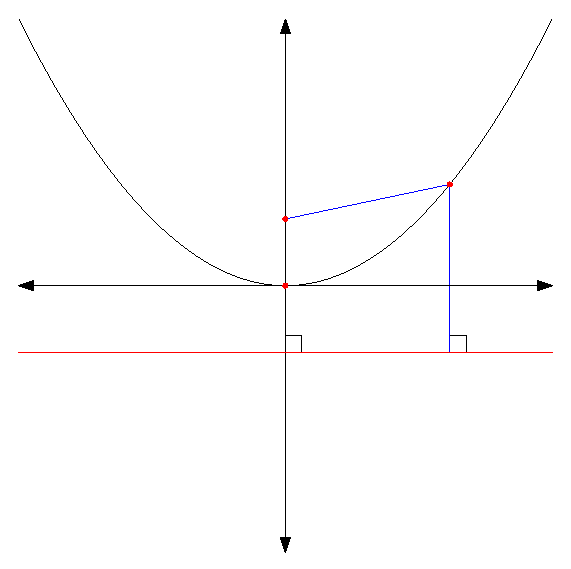
\includegraphics{./parab_x_orig}
\end{frame}


\begin{frame}[label={sec:orga2b2941}]{The Parabola}
\end{frame}

\begin{frame}[label={sec:org85b1a05}]{The Parabola}
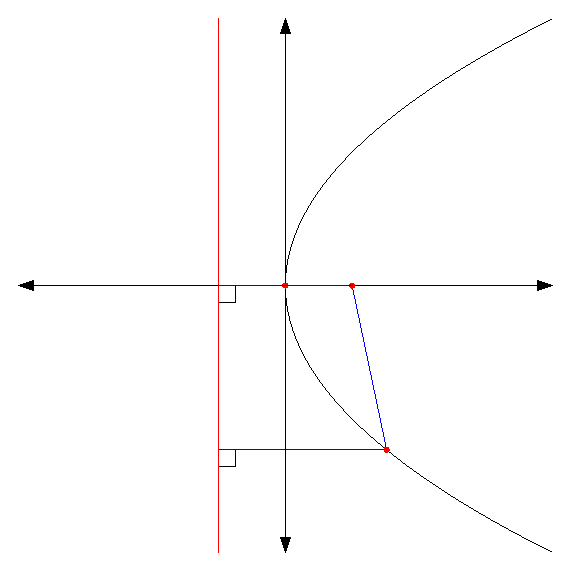
\includegraphics{./parab_y_orig}
\end{frame}

\begin{frame}[label={sec:org87277ed}]{The Parabola}
\begin{center}
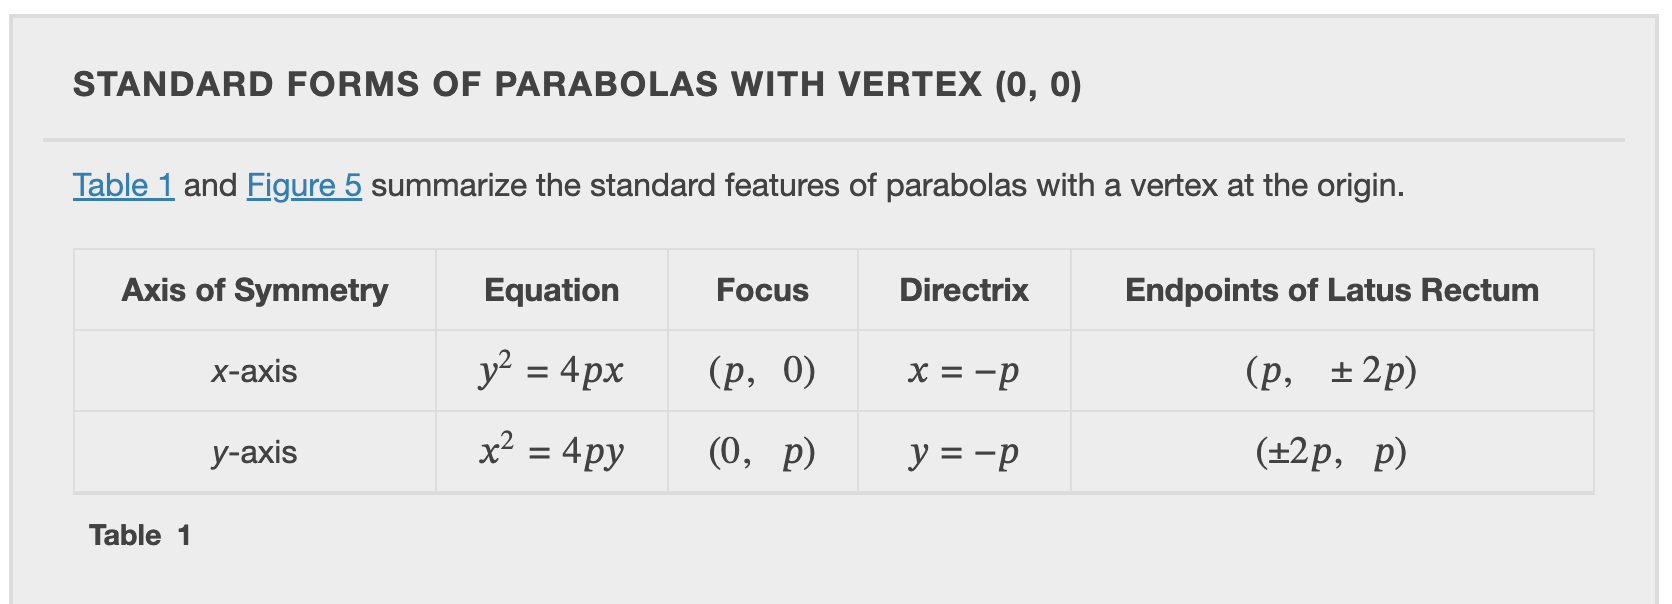
\includegraphics[width=0.8\textwidth]{./parabs_origin}
\end{center}
\end{frame}

\begin{frame}[label={sec:org27f86c3}]{Example}
Graph
\[
8y = x^2\]

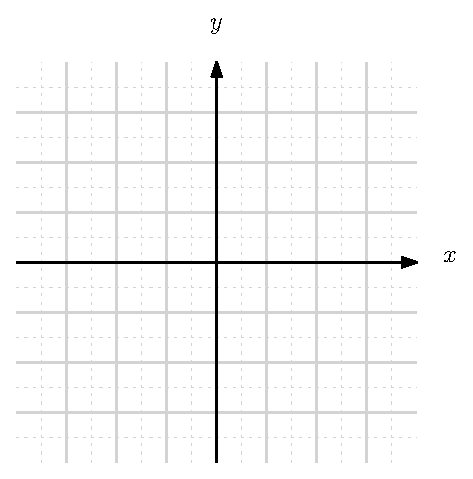
\includegraphics[scale=0.9]{./blank_grid}
\vspace{10in}
\end{frame}


\begin{frame}[label={sec:org4c185e7}]{Example}
Graph
\[
16x = y^2\]

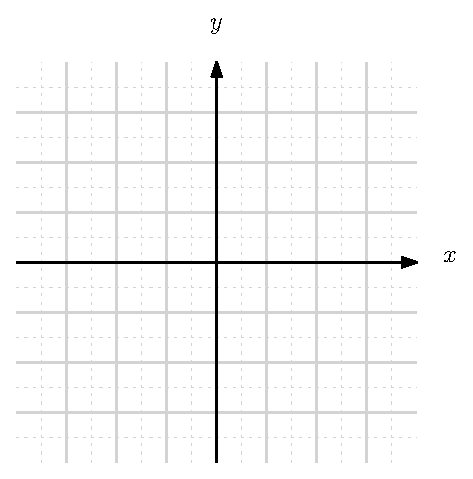
\includegraphics[scale=0.9]{./blank_grid}
\vspace{10in}
\end{frame}


\begin{frame}[label={sec:orgb5782c0}]{Example}
What is the equation of a parabola that has a focus of \(\left(
-\frac{1}{2},0 \right)\) and a directrix \(x = \frac{1}{2}?\)

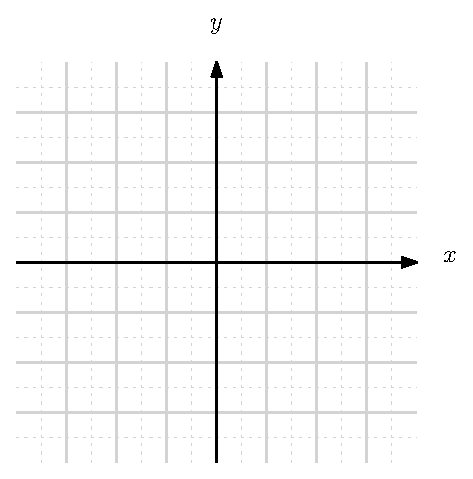
\includegraphics[scale=0.9]{./blank_grid}
\vspace{10in}
\end{frame}
\end{document}